\begin{exercice}[Diagramme en bâtons]
Pour fabriquer du chocolat noir, il faut mélanger de la pâte de cacao et du sucre. Dans une pâtisserie, on a relevé les quantités de pâte de cacao et de sucre utilisées les cinq derniers mois dans le graphique ci‑dessous :
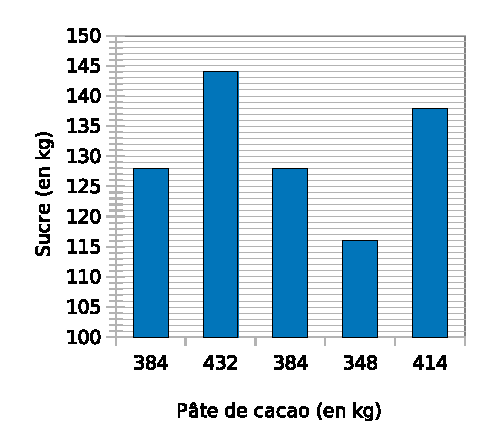
\includegraphics[width=7.7cm]{diag_batons}
\begin{enumerate}
 \item Recopie et complète à l'aide des données du graphique, un tableau comme celui proposé ci‑dessous :
 \vspace{0.5cm}
 \begin{minipage}[c]{0.86\linewidth}
  \begin{tabularx}{\linewidth}{|c|*{4}{>{\centering\arraybackslash}X|}}
  \hline
 \cellcolor{J2} Masse de sucre (en kg) & & & \\\hline
 \cellcolor{J2} Masse de pâte de cacao (en kg) & & & \\\hline
 \end{tabularx}
\end{minipage} \hfill%
 \begin{minipage}[c]{0.1\linewidth}
\vspace{0.5cm}
\ldots

\ldots
\end{minipage} \\
 \item D'après ce tableau, peut‑on dire que la masse de sucre est proportionnelle à celle de la pâte de cacao ? Justifie ta réponse.
 \end{enumerate}
\end{exercice}


\begin{exercice}[Des mélanges]
Une entreprise propose plusieurs types de béton selon la quantité de gravier, de sable et de ciment qu'il comporte.
\begin{center}
 \renewcommand*\tabularxcolumn[1]{>{\centering\arraybackslash}m{#1}}
 \begin{ttableau}{\linewidth}{4}
 \hline
 & \cellcolor{BleuOuv} Gravier & \cellcolor{BleuOuv} Sable & \cellcolor{BleuOuv} Ciment \\\hline
 \cellcolor{BleuOuv} Béton A & 21 kg & 10 kg & 9 kg \\\hline
 \cellcolor{BleuOuv} Béton B & 9 kg & 3,5 kg & 3 kg \\\hline
 \cellcolor{BleuOuv} Béton C & 11 kg & 8,5 kg & 9,5 kg \\\hline
 \end{ttableau}
\end{center}
Parmi ces mélanges, quel est celui qui comporte : 
\begin{enumerate}
 \item La plus grande proportion de gravier ? 
 \item La plus grande proportion de sable ? 
 \item La plus grande proportion de ciment ? 
 \end{enumerate}
Tu justifieras chacune de tes réponses.
\end{exercice}


\begin{exercice}[Diagramme circulaire]
Dans le collège Sésacol, la répartition des élèves en fonction du niveau est la suivante :
\begin{center}
 \begin{tabularx}{\linewidth}{|c|*{4}{>{\centering\arraybackslash}X|}}
  \hline
  \rowcolor{U2} Niveau & 5\up{ème} & 6\up{ème} & 7\up{ème} & 8\up{ème} \\\hline
  \rowcolor{C3} Nombre d'élèves & 126 & 112 & 120 & 122 \\\hline
  \end{tabularx}
 \end{center}
On souhaite représenter ces données à l'aide d'un diagramme circulaire.
\begin{enumerate}
 \item Combien y a‑t‑il d'élèves dans ce collège ? Quelle est la mesure de l'angle au centre d'un secteur angulaire qui représenterait l'ensemble des élèves de ce collège dans un diagramme circulaire ?
 \item Recopie et complète le tableau de proportionnalité suivant :
\vspace{0.3cm}
\begin{center}
 \begin{tabularx}{\linewidth}{|c|*{5}{>{\centering\arraybackslash}X|}}
  \hline
  \rowcolor{U2} Niveau & 6\up{ème} & 5\up{ème} & 4\up{ème} & 3\up{ème} & Total \\\hline
  \rowcolor{C3} Nombre d'élèves & 126 & 112 & 120 & 122 & \\\hline
  \rowcolor{F3} Angle au centre & & & & & $360^\circ$ \\\hline
  \end{tabularx}
 \end{center}
 \vspace{0.3cm}
 \item Trace un cercle de rayon 5 cm et représente la répartition des élèves sous forme de diagramme circulaire.
 \end{enumerate}
\end{exercice}

